\documentclass{article}

\usepackage{cancel}
\usepackage{tikz}
\usepackage{amsmath}
\usepackage{geometry}
\usepackage{graphicx}
\usepackage{amsfonts} 
\usepackage{verbatim}
\usepackage{mathrsfs}  
\usepackage{lmodern}
\usepackage{braket}
\usepackage{bookmark}


\usetikzlibrary{petri, positioning}
\hypersetup{
    colorlinks=true,
    linkcolor=black,
}

\tikzset{every transition/.style={draw,minimum width=1mm,minimum height=5mm},
         every place/.style={draw,thick,minimum size=6mm},
         ltransition/.style={draw,minimum width=5mm,minimum height=1mm}}

\renewcommand{\contentsname}{Indice}

\numberwithin{equation}{subsection}

\title{Appunti di Analisi dei Sistemi ad Eventi}
\author{Giacomo Sturm}
\date{AA: 2023/2024 - Ing. Informatica}

\begin{document}

\maketitle

\vspace{10mm}

\begin{center}
    Sorgente del file LaTeX disponibile su \url{https://github.com/00Darxk/Analisi-dei-Sistemi-ad-Eventi}
\end{center}

\clearpage

\tableofcontents

\clearpage

\section{Introduzione}

Verrano forniti due modelli di sistemi, reali o astratti, un modello matematico, reti di Code, ed un modello logico, reti di Petri. Quest'ultimo è un modello grafico, simile ad 
un diagramma di flusso. La rete di Petri analizza le interazioni tra gli elementi del sistema, mentre la rete di Code analizza nel tempo queste interazioni ingresso-uscita. 
In questi modelli si analizza l'evoluzione di una variabile di stato, da individuare nel sistema analizzato, per studiare la funzione obiettivo. La variazione della variabile 
di stato si studia tramite derivata continua o discreta, oppure si campiona il suo valore ad intervalli fissi. L'analisi ad eventi consiste nel misurare solamente se succede 
qualcosa al sistema, se avviene un evento, ovvero non c'è spreco di memoria campionando lo stesso valore. Per determinare un evento si controlla se la variabile di stato 
considerata è cambiata, questa variabile può essere sia deterministica oppure aleatoria. In caso sia aleatoria, conoscere la sua distribuzione di probabilità non è sufficiente 
per determinarne l'evouzione, sono necessaria la media, il valore centrale della distribuzione, e la varianza, la distanza dal valore centrale nella distribuzione. 



Si usano sistemi manufatturieri come esempi, poiché sono comuni e seplici da studiare. Viene definita una coda un luogo dove i clienti o utenti aspettano il servizio. Quando un 
cliente entra nel sistema, se è disponibile un servente, viene servito, se non è disponibile si mette in coda. Viene definito tempo di processamento il tempo 
necessario per un cliente affinché sia servito. Si considerano i clienti usciti dal sistema dopo essere stati serviti. Si considera per ipotesi la coda ordinate in FIFO (First 
In First Out), ovvero si considera il primo cliente entrato in coda, il primo servito, se sono disponibili serventi. La coda del modello può essere illimitata oppure 
limitata con un massimo numero clienti $k$. Si indica il numero dei serventi con $s$. Si definisce la variabile di stato di questo sistema il valore intero $n$ che 
rappresenta il numero di clienti all'interno del sistema, il suo valore massimo corrisponde alla massima capienza dei servneti e della coda: $n\in[0,s+k]$. Questo valore 
si incremente o decrementa di uno ogni volta che un cliente entra o esce dal sistema. In uno stesso istante non può avvenire più di un evento, ovvero la variabile può 
variare di uno in ogni istante. Si chiamano questi eventi di incremento e decremento processi di nascita e morte. Questo sistema è descritto da una legge di transizione:
\begin{equation*}
    \begin{cases}
        n=n+1\\
        n=n-1
    \end{cases}
\end{equation*}
Quest'equazione rappresenta la legge di evoluzione del sistema. Un evento rappresenta l'arrivo o la partenza di un cliente dal sistema. In questo modello la variazione è slegata 
dal tempo, noto solo il cambiamento della variabile di stato ad ogni evento, per cui rappresenta un modello logico. Se ad ogni evento viene assegnato una durata di tempo il 
modello diventa temporizzato, in maniera asincrona, ovvero ogni evento corrisponde ad intervalli di tempo diversi. L'obiettivo del modello è determinare l'evoluzione del sistema, 
questo può comprendere il numero di clienti, il tempo di servizio, differenza tra il tempo di entrata ed il tempo di uscita di un cliente, il tempo di attesa. Conoscendo il 
tempo di processamento si può deterinare se il sistemaè sotto o sovra-utilizzato.

\clearpage

\section{Reti di Petri}

La rete di Petri è un modello logico per rappresentare sistemi ad eventi deterministici (DES), può rappresentare comportamenti complessi come la sincronizzazione, il succedersi 
asincrono di eventi che avvengono in intervalli di tempo diversi, operazioni concorrenti che avvengono totalemente indipendentemente tra di loro, conflitti ed altre 
caratteristiche di sistemi ad eventi. 

\subsection{Rappresentazione}

La rete di petri è una rappresentazione grafica con una struttura matematica, è modulare e limitata, potendo rappresentare un ciclo continuo, è possibile gestire il ridimensionamento 
della rete senza perdere le sue proprietà. La rete è un grafo bipartito, formato da due tipi di nodi, i posti $p$ e le transizioni $t$. Si possono unire solamente posti-transizioni 
tramite archi orientati. 
\begin{center}
    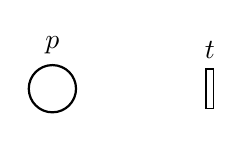
\begin{tikzpicture}
        \node[place, label=above:$p$](p)at(0,0){};
        \node[transition, label=above:$t$](t)at(2,0){};
    \end{tikzpicture}
\end{center}
Viene definito pre-set di un nodo $x$ l'insieme dei nodi immediatamente a monte di $x$: $\bullet x$, viene invece definito post-set di un nodo $x$ l'insieme dei nodi 
immediatamente a valle di $x$: $x\bullet$. Lo stato del sistema viene definito dalla marcatura $x$ un vettore colonna di dimensione pari al numero di posti $|P|$, dove $P$ 
indica l'insieme dei posti, ed avente ogni componente di valore uguale al numero di gettoni presenti nel posto associato:
\begin{equation*}
    x=\begin{pmatrix}
        x_1\\
        \vdots\\
        x_{|P|}
    \end{pmatrix}
\end{equation*}
Viene definita marcatura iniziale $x_0$ lo stato assunto dal sistema all'inizio della sua analisi. 
I nodi sono collegati da archi pesati, il peso di un arco esprime il numero di gettoni generati, in caso sia in entrata ad un posto, oppure consumati, in caso sia in entrata 
ad una transizione. Il peso di un arco può essere indicato come un numero espresso sopra l'arco, per convenzione se è omesso il peso si considera di peso unitario, oppure 
si possono rappresentare come un numero di archi pari al peso dell'arco:
\begin{center}
    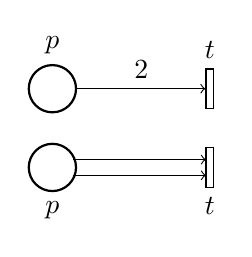
\begin{tikzpicture}
        \node[place, label=above:$p$](p1)at(0,0){};
        \node[transition, label=above:$t$](t1)at(2,0){};
        \draw[->](p1.0)--(t1.180)node[midway, above]{$2$};

        \draw[->](0.26,-0.9)--(1.95,-0.9);
        \draw[->](0.26,-1.1)--(1.95,-1.1);
        \node[place, label=below:$p$](p2)at(0,-1){};
        \node[transition, label=below:$t$](t2)at(2,-1){};
    \end{tikzpicture}
\end{center}

\subsubsection{Evoluzione}

Una transizione è abilitata se i posti a monte della transizione contengono almeno abbastanza gettoni da poter essere tutti consumati dai rispettivi archi. 

\begin{center}
    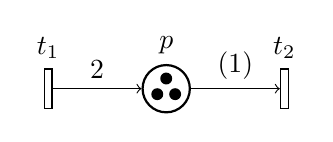
\begin{tikzpicture}
        \node[transition, label=above:$t_1$](t1)at(-0.5,0){};
        \node[place,tokens=3,label=above:$p$](p)at(1,0){};
        \node[transition,label=above:$t_2$](t2)at(2.5,0){};
        \draw[->](t1.0)--(p.180)node[midway, above]{$2$};
        \draw[->](p.0)--(t2.180)node[midway, above]{$(1)$};
    \end{tikzpicture}
\end{center}

In questo esempio la transizione $t_2$ è abilitata, poiché l'arco consuma tre gettoni e nel posto immediatamente a monte della transizione sono presenti tre gettoni. 
Ad ogni transizione può essere associato un tempo di processamento, in modo da temmporizzare il sistema. Se il pre-set di una transizione è vuoto, allora quella transizione 
è sempre abilitata. 

Il numero di stati possibili in una qualsiasi configurazione corrisponde al numero di transizioni abilitate in quella data configurazione. Questi stati possibili possono 
essere rappresentati con un grafo di stato, in base alla rete e alla marcatura iniziale considerata $x_0$. 

Si definiscono posti con un pre-set nullo appesi ed il numero di gettoni al loro interno può o rimanere costante o diminuire. Per cui se il sistema si basa solamente su posti 
appesi, allora sicuramente si bloccherà, incontra un "deadlock". 


L'evoluzione di un sistema viene determinata dall'accadimento di eventi abilitati, ognuno con una sua abilità di accadere. La possibilità che un evento accada dipende dall'
abilitazione di una transizione, l'effetto del suo accadimento corrisponde allo scatto di una transizione. L'abilitazione di una transizione dipende solamente dal peso dell'
arco in entrata e dai gettoni nel pre-set, è abilitata se il numero dei gettoni nel pre-set è almeno uguale al peso dei rispettivi archi. 
Lo scatto di una transizione provoca un "flusso" di gettoni, questo flusso non è continuo, poiché i gettoni in entrata alla transizione vengono consumati e ne vengono creati 
di nuovi sulla base del peso dell'arco in uscita, numero indipendente dal numero dei gettoni consumati. 

L'evoluzione comprende quattro passaggi ciclici: data una marcatura corrente si individua l'insieme delle transizioni abilitate, si sceglie casualmente, se non è specificato, 
una sola di queste transizioni, si provoca lo scatto di questa transizione che cambia la marcatura, si considera la nuova marcatura corrente e si ripetono questi passaggi. 

Una sequenza di transizioni, abilitate, $(t_1,\cdots,t_n)$ si esprime con il simbolo $S$. Questa sequenza rappresenta l'ordine con cui le transizioni scattano, affinché 
rappresenti una sequenza valida, le transizioni considerate devono essere abilitate quando è il loro turno di scattare. Diverse sequenze possono arrivare alla stessa 
marcatura. 
Un singolo posto può abilitare più di una transizione, ma dopo lo scatto di una delle transizioni abilitate, potrebbe non avere gettoni rimanenti per abilitare le altre. 

\subsubsection{Strutture Fondamentali}

Due transizioni si dicono in sequenza se sono collegate da un singolo posto:
\begin{center}
    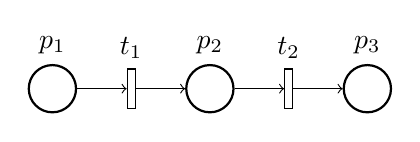
\begin{tikzpicture}
        \node[place, label=above:$p_1$](p1)at(0,0){};
        \node[transition, label=above:$t_1$](t1)at(1,0){};
        \node[place, label=above:$p_2$](p2)at(2,0){};
        \node[transition, label=above:$t_2$](t2)at(3,0){};
        \node[place, label=above:$p_3$](p3)at(4,0){};

        \draw[->](p1.0)--(t1.180);
        \draw[->](t1.0)--(p2.180);
        \draw[->](p2.0)--(t2.180);
        \draw[->](t2.0)--(p3.180);
    \end{tikzpicture}
\end{center}
Le transizioni $t_1$ e $t_2$ si dicono in sequenza. 


Un posto d'ingresso a due o più transizioni rappresenta un conflitto strutturale. Questo conflitto può essere effettivo se data una marcatura $M$, lo scatto di una transizione 
disabilita le altre transizioni. Il conflitto è potenziale se questo scatto non disabilita le altre transizioni. 
\begin{center}
    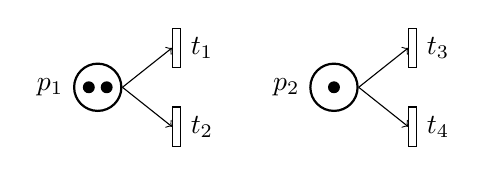
\begin{tikzpicture}
        \node[place, tokens=2, label=left:$p_1$](p1)at(0,0){};
        \node[transition, label=right:$t_1$](t1)at(1,0.5){};
        \node[transition, label=right:$t_2$](t2)at(1,-0.5){};

        \draw[->](p1.0)--(t1.180);
        \draw[->](p1.0)--(t2.180);

        \node[place, tokens=1, label=left:$p_2$](p2)at(3,0){};
        \node[transition, label=right:$t_3$](t3)at(4,0.5){};
        \node[transition, label=right:$t_4$](t4)at(4,-0.5){};

        \draw[->](p2.0)--(t3.180);
        \draw[->](p2.0)--(t4.180);
    \end{tikzpicture}
\end{center}
Le transizioni $t_1$ e $t_2$ si dicono in conflitto potenziale, le $t_3$ e $t_4$ si dicono in conflitto effettivo. 


Due, o più, transizioni si dicono concorrenti se la loro evoluzione è indipendente l'una dall'altra:
\begin{center}
    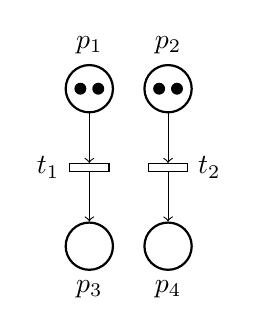
\begin{tikzpicture}
        \node[place, tokens=2, label=above:$p_1$](p1)at(0,0){};
        \node[place, tokens=2, label=above:$p_2$](p2)at(1,0){};
        \node[transition, rotate=90,label=above:$t_1$](t1)at(0,-1){};
        \node[transition, rotate=90,label=below:$t_2$](t2)at(1,-1){};
        \node[place, label=below:$p_3$](p3)at(0,-2){};
        \node[place, label=below:$p_4$](p4)at(1,-2){};

        \draw[->](p1.270)--(t1.0);
        \draw[->](p2.270)--(t2.0);
        \draw[<-](p3.90)--(t1.180);
        \draw[<-](p4.90)--(t2.180);
    \end{tikzpicture}
\end{center}
Le transizioni $t_1$ e $t_2$ si dicono in concorrenza strutturale, essendo entrambe abilitate si dicono in concorrenza effettiva. 



Due o più posti si dicono sincronizzati se come post-set presentano la stessa transizione:
\begin{center}
    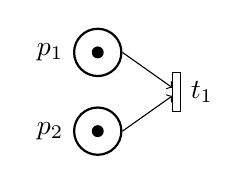
\begin{tikzpicture}
        \node[place, tokens=1, label=left:$p_1$](p1)at(0,0.5){};
        \node[place, tokens=1, label=left:$p_2$](p2)at(0,-0.5){};
        \node[transition, label=right:$t_1$](t1)at(1,0){};

        \draw[->](p1.0)--(0.95,0.05);
        \draw[->](p2.0)--(0.95,-0.05);
    \end{tikzpicture}
\end{center}
I posti $p_1$ e $p_2$ si dicono sincronizzati tra di loro, la transizione $t$ si identifica come transizione di sincronizzazione


Due o più posti si dicono concorrenti se presentano in pre-set la stessa transizione, per cui allo scatto di quella transizione vengono generati dei gettoni in entrambi i posti:
\begin{center}
    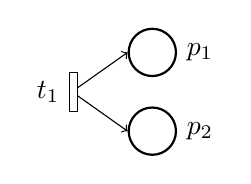
\begin{tikzpicture}
        \node[place, label=right:$p_1$](p1)at(1,0.5){};
        \node[place, label=right:$p_2$](p2)at(1,-0.5){};
        \node[transition, label=left:$t_1$](t1)at(0,0){};
        
        \draw[->](0.05,0.05)--(p1.180);
        \draw[->](0.05,-0.05)--(p2.180);
    \end{tikzpicture}
\end{center}
I due posti $p_1$ e $p_2$ si dicono concorrenti tra di loro, la transzizione $t$ si identifica come transizione di inizio concorrenza. 


Una rete di Petri si dice completa se non presenta nessun posto e transizione appese. 

\subsubsection{Sistema Produttori/Consumatori}

Si considera un sistema semplice formato da uno o più produttori che creano oggetti e li depositano in un buffer condiviso da cui uno o più consumatori possono prelevarli 
e consumarli. Per rappresentare un consumatore o un produttore si un ciclo che produce uno o più gettoni e lo depositano in un posto esterno al ciclo, oppure  prelevano uno o 
più gettoni per poi consumarli con lo scatto di una transizione del ciclo:

\begin{center}
    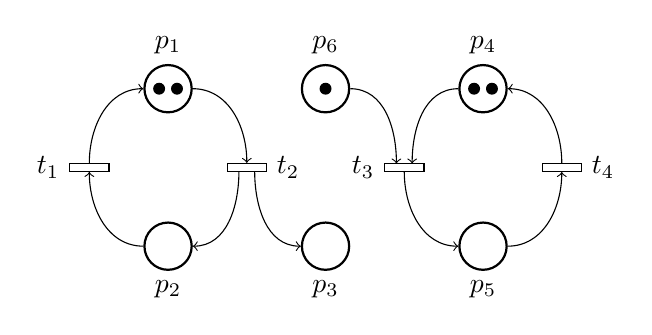
\begin{tikzpicture}
        \node[place, tokens=2, label=above:$p_1$](p1)at(0,1){};
        \node[place, label=below:$p_2$](p2)at(0,-1){};
        \node[transition, rotate=90, label=below:$t_2$](t2)at(1,0){};
        \node[transition, rotate=90, label=above:$t_1$](t1)at(-1,0){};
        \draw[->](p1.0)to [out=0,in=90](t2.0);
        \draw[->](0.9,-0.05)to [out=270,in=0](p2.0);
        \draw[->](p2.180)to [out=180,in=270](t1.180);
        \draw[->](t1.0)to [out=90,in=180](p1.180);

        \node[place, label=below:$p_3$](p3)at(2,-1){};
        \draw[->](1.1,-0.05)to[out=270,in=180](p3.180);
        
        \node[place, tokens=2, label=above:$p_4$](p4)at(4,1){};
        \node[place, label=below:$p_5$](p5)at(4,-1){};
        \node[transition, rotate=90, label=below:$t_4$](t4)at(5,0){};
        \node[transition, rotate=90, label=above:$t_3$](t3)at(3,0){};
        \draw[<-](p4.0)to [out=0,in=90](t4.0);
        \draw[<-](t4.180)to [out=270,in=0](p5.0);
        \draw[<-](p5.180)to [out=180,in=270](t3.180);
        \draw[<-](3.1,0.05)to [out=90,in=180](p4.180);

        \node[place, tokens=1,label=above:$p_6$](p6)at(2,1){};
        \draw[->](p6.0)to[out=0,in=90](2.9,0.05);
    \end{tikzpicture}
\end{center}

In questo caso ogni volta che la transizione $t_2$ scatta, viene generato un gettone nel posto $p_3$, quindi il ciclo rappresenta un ciclo di produttori ed il numero di 
gettoni nel ciclo, indica il numero di produttori. La transizione $t_3$ è abilitata solo se è presente almeno un gettone nel posto $p_6$, per cui questo ciclo 
consuma un gettone ogni volta che scatta $t_6$, rappresenta un ciclo di consumatori, ed il numero di gettoni nel ciclo rappresenta il numero di consumatori del sistema. 
In un qualsiasi ciclo il numero di gettoni rimane sempre costante, se il peso degli archi che generano gettoni è uguale al peso dei gettoni che consumano gettoni, e se le 
transizioni sono sempre abilitate, altrimenti il ciclo non potrebbe né consumare né generare gettoni. 

Per creare un sistema unico produttori-consumatori si considera un posto dove vengono depositati i gettoni generati dal ciclo dei produttori e consumati dal ciclo dei 
consumatori. Questo deposito può essere sia illimitato, nelle situazioni precedenti, oppure limitato. In questo caso è necessario un controllo nelle transizioni pre-set 
del buffer per impedire siano generatati gettoni se il deposito non può accomodarli, analogamente è necessario un controllo post-set per segnalare che un numero di gettoni è 
diminuito e quindi il deposito può accomodare più gettoni. Per indicare questo limite si crea un ciclo composto dalle transizioni generatrici nel cicli dei produttori, 
il posto buffer, le transizioni consumatrici dei cicli dei consumatori, ed un altro poste. In questo ciclo così definito il numero di gettoni rimane invariato, per cui il 
massimo numero di gettoni presenti nel deposito non può eccedere un limite imposto a priori:


\begin{center}
    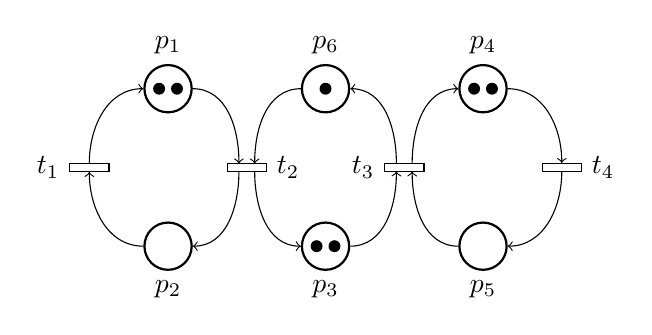
\begin{tikzpicture}
        \node[place, tokens=2, label=above:$p_1$](p1)at(0,1){};
        \node[place, label=below:$p_2$](p2)at(0,-1){};
        \node[transition, rotate=90, label=below:$t_2$](t2)at(1,0){};
        \node[transition, rotate=90, label=above:$t_1$](t1)at(-1,0){};
        \draw[->](p1.0)to [out=0,in=90](0.9,0.05);
        \draw[->](0.9,-0.05)to [out=270,in=0](p2.0);
        \draw[->](p2.180)to [out=180,in=270](t1.180);
        \draw[->](t1.0)to [out=90,in=180](p1.180);

        \node[place, tokens=2,label=below:$p_3$](p3)at(2,-1){};
        \draw[->](1.1,-0.05)to[out=270,in=180](p3.180);
        
        \node[place, tokens=2, label=above:$p_4$](p4)at(4,1){};
        \node[place, label=below:$p_5$](p5)at(4,-1){};
        \node[transition, rotate=90, label=below:$t_4$](t4)at(5,0){};
        \node[transition, rotate=90, label=above:$t_3$](t3)at(3,0){};
        \draw[->](p4.0)to [out=0,in=90](t4.0);
        \draw[->](t4.180)to [out=270,in=0](p5.0);
        \draw[->](p5.180)to [out=180,in=270](3.1,-0.05);
        \draw[->](3.1,0.05)to [out=90,in=180](p4.180);

        \node[place, tokens=1,label=above:$p_6$](p6)at(2,1){};
        \draw[<-](p6.0)to[out=0,in=90](2.9,0.05);
        \draw[->](p3.0)to[out=0,in=270](2.9,-0.05);
        \draw[->](p6.180)to[out=180,in=90](1.1,0.05);
    \end{tikzpicture}
\end{center}

In questo caso il deposito presenta un limite massimo di tre gettoni, e nel sistema sono presenti due consumatori e due produttori. Generalmente modelli di sistemi di produttori 
e consumatori presentano sempre dei cicli simili comunicanti tra di loro. 

\subsection{Proprietà}

Una stessa rete presenta proprietà diverse in base ad una diversa marcatura iniziale $M_0$. 

\subsubsection{Raggiungibilità}
Una marcatura $M^*$ si dice raggiugibile se esiste almeno una sequenza $S$ di transizioni abilitate tale che sia possibile, da una marcatura iniziale $M$, raggiungere la 
marcatura $M^*$:
\begin{equation*}
    M\left[S>M^*\right.
\end{equation*}


Si definisce, data una rete di Petri $N$ marcata con una marcatura $M_0$, l'insieme di raggiungibilità $R(N,M_0)$, l'insieme più piccolo di marcature tale che la marcatura 
iniziale appartiene all'insieme, e data una qualsiasi marcatura $M^*$ appartenente all'insieme, ed una qualsiasi transizione $t$, abilitata, appartenente all'insisme delle transizioni 
$T$ nella marcatura $M^*$. La transizione $M^{**}$ ottenuta facendo scattare la transizione $t$ nella marcatura $M^*$ anch'essa appartiene all'insieme di raggiungibilità. 
\begin{align*}
    &M_0\in R(N,M_0)\\
    &M^*\in R(N,M_0)\land t\in T\mbox{ t.c. } M^*\left[\right.t>M^{**}\implies M^{**}\in R(N,M_0)
\end{align*}

\subsubsection{Limitatezza}

Un posto $p_i$ di una rete $N$ si dice $k-$limitato se in tutte le marcature raggiungibili, da una marcatura iniziale $M_0$, quel posto presenta al massimo $k$ gettoni al 
suo interno:
\begin{equation*}
    \forall M\in R(N,M_0)\to m_i\leq k
\end{equation*} 
Una rete $N$ in una marcatura iniziale $M_0$ si dice $k-$limitata se tutti i suoi posti sono $k-$limitati. Se $k=1$, la rete si dice binaria, poiché ogni 
posto può avere o zero o un singolo gettone. Una rete si dice limitata al massimo numero di gettoni che possono esistere in uno dei suoi posti, per cui è sufficiente un 
singolo posto illimitato affinché l'intera rete sia illimitata. 

I cicli, analizzati precedentemente, rappresentano un caso semplice di rete limitata, poiché il numero di gettoni presenti nel ciclo rimane costante. 

\subsubsection{Reversibilità}

Una rete $N$ si dice reversibile, a partire da una marcatura iniziale $M_0$, se per ogni marcatura $M$ appartenente all'insieme di raggiungibilià, la marcatura iniziale 
appartiene all'insieme di raggiungibilità della marcatura $M$:
\begin{equation*}
    \forall M\in R(N,M_0)\implies M_0\in R(N,M)
\end{equation*}
Per cui una rete si dice reversibile se per ogni marcatura $M$ raggiungibile deve esistere una serie di scatti $S$ tali da ritornare alla marcatura originale $M_0$:
\begin{equation*}
    \forall M\in R(N,M_0)\implies M\left[\right.S>M_0
\end{equation*} 

\subsubsection{Conservatitivà}

Una rete $N$ con marcatura iniziale $M_0$ si dice conservativa in riferimento ad un vettore peso $W$ (colonna), maggiore uguale al vettore nullo $0$, di dimensione pari alla 
cardinalità dell'insieme dei posti $\mbox{dim} W=|P|$, se per ogni marcatura $M$ appartenente all'insieme di raggiungibilità $R$ il prodotto matriciale tra la trasposta del 
vettore peso $W$ ed il vettore marcatura $M$ assume un valore finito e costante:
\begin{equation*}
    \exists W\geq0\mbox{ t.c. }\forall M\in R(N,M_0)\implies W^T\cdot M=k\in\mathbb{R}^+
\end{equation*}


Il vettore peso $W$ poiché è maggiore uguale al vettore nullo presente al minimo una sola componente non nulla positiva, ed al massimo tutte componenti positive non nulle. Il 
prodotto tra $W^T$ e $M$ si può esprimere in diversi modi:
\begin{gather*}
    \forall M\in R(N,M_0):\,W^T\cdot M=\begin{bmatrix}
        w_1,\cdots,w_{|P|}
    \end{bmatrix}\cdot\begin{pmatrix}
        m_1\\
        \vdots\\
        m_{|P|}
    \end{pmatrix}=\displaystyle\sum_{j=1}^{|P|}w_jm_j=k\\
    M_0\in R(N,M_0)\implies W^T\cdot M=W^T\cdot M_0=k\\
    \displaystyle\sum_{j=1}^{|P|}w_jm_j=\sum_{j=1}^{|P|}w_jm_{j0}\to \sum_{j=1}^{|P|}w_j(m_j-m_{j0})=0
\end{gather*}


Una rete si dice conservativa, se esiste un vettore peso $W$ strettamente maggiore del vettore nullo, per cui il prodotto la trasposta del vettore ed una qualsiasi marcatura 
appartenente all'insieme di raggiungibilità risulta sempre costante:
\begin{equation*}
    \exists W>0\mbox{ t.c }\forall M\in R(N,M_0)\implies W^T\cdot M=k\in\mathbb{R}^+
\end{equation*}
Una rete conservativà quindi è $k-$limitata poiché non è necessario azzerare il contributo di un posto, a differenza del caso della conservativà in riferimento ad un vettore 
dove il vettore $W$ contiene tanti zeri quanti sono i posti illimitati nella rete $N$, in modo da azzerare i loro contriubti nella somma. 

Una rete si dice strettamente conservativa se è conservativa con riferimento al vettore identità, per cui tutte le componenti del vettore peso $W$ assumono valore unitario: 
$\forall j\in\,1,\cdots,|P|\implies w_j=1$. 


Una rete si dice non conservativa se è conservativa con riferimento ad un vettore peso nullo, per cui tutti i suoi posti sono illimitati, per cui il numero di posti rimane 
costante solo se non si considera nessun posto della rete. 

In generale per controllare la conservatività si cerca il sottoinsieme più grande dell'insieme dei posti della rete $N$ dove il numero di gettoni rimane complessivamente 
costante. Si deduce quindi che un ciclo rappresenta un elemeno conservativo, e se è presente in una rete, sarà sempre conservativà rispetto ad un vettore, se i posti del ciclo 
presentano almeno un vettore. 

\subsubsection{Vivezza}

Una transizione $t$, di una rete $N$ con marcatura iniziale $M_0$, si dice viva, se e solo se per ogni marcatura $M$ appartenente all'insieme di raggiungibilità $R$ esiste una 
marcaura $M^*$ raggiungibile da $M$, tale che la transizione $t$ sia abilitata:
\begin{equation*}
    t:\mbox{viva}\iff \forall M\in R(N,M_0),\,\exists M^*\in R(N,M)\mbox{ t.c. } t:\mbox{abilitata in }M^*
\end{equation*}
Una rete $N$, con marcatura iniziale $M_0$, si dice raggiungibile se e solo se tutte le sue transizioni $t_j$ sono vive:
\begin{equation*}
    N:\mbox{viva}\iff \forall t\in T\to t:\mbox{viva} 
\end{equation*}

\subsection{Analisi Dimamica e Strutturale}

Partendo da una rete è possibile creare un grafo di stato o grafo di raggiungibilità, che racchiude le relazioni tra ogni marcatura appartenente all'insieme di raggiungibilità, 
data una marcatura iniziale $M_0$, tramite li scatti di una singola transizione. Questo grafo è sempre limitato, anche se la rete non lo è. Dal grafo è possible inferire sulle 
proprietà della rete in quella data configurazione. 
Bisogna tenere conto delle differenza tra le prorpietà strutturali di una rete, che non dipendono dalla marcatura iniziale $M_0$, e le proprietà dinamiche che dipedono dalla 
marcatura $M_0$. Le proprietà individuate da un'analisi strutturale sono più importanti poiché intrinseche alla rete e verrano studiate nelle sezioni successive. 

\subsubsection{Grafo di Raggiungibilità e di Copertura}

Un grafo di raggiungibilità è un grafo con un unico tipo di nodo che corrisponde ad una marcatura $M$. Sono presenti tanti nodi quante sono le marcature presenti nell'insieme 
di raggiungibilità $R$, a partire da una marcatura iniziale $M_0$. Gli archi del grafo uniscono due marcature collegate dallo scatto di una singola transizione, abilitata. 
Se è presente un numero finito di nodi, la rete è limitata, se sono presenti solo valori di $0$ e $1$, allora la rete è binaria. Se da ogni nodo del grafo esiste un percorso 
che abilita tutte le transizioni allora la rete è viva. Se da ogni nodo esiste un percorso che ritorna allo stesso nodo, la rete è reversibile. 
\\
Per costruire un grafo di raggiungibilità si parte dalla marcatura iniziale $M_0$, segnandola come nodo corrente. Si indica $M_k$ la marcatura associata al nodo corrente; 
se non ci sono più transizioni attivabili a partire dal nodo corrente, non considerate in precedenza rispetto allo stesso nodo, e se il nodo corrente non corrisponde alla 
marcatura iniziale $k>0$ allora si assegna come nodo corrente $M_{k-1}$, altrimeni l'algoritmo termina. Si considera la prima transizione abilitata, non considerata in precedenza 
con riferimento allo stesso nodo, e si calcola la marcatura raggiunta dal suo scatto. Se questa marcatura non corrisponde ad una marcatura già analizzata la si chiama $M_{k+1}$, 
e si crea un nodo associato ad essa collegato al nodo corrente da un arco, indicando la transizione scattata per arrivarci. Questo nodo diventa il nuovo nodo corrente e si 
ricomincia l'algoritmo cercando transizioni attivabili a partire da questo nodo corrente.  
\begin{center}
    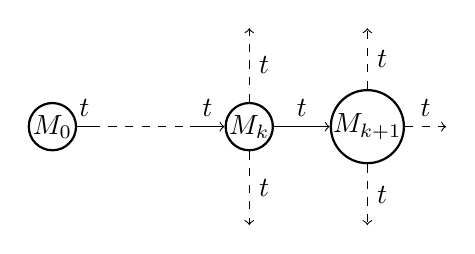
\begin{tikzpicture}
        \node[place](p1)at(-1,0){$M_0$};
        \draw[-](p1.0)--(-0.5,0)node[midway, above]{$t$};
        \draw[dashed](-0.5,0)--(0.75,0);

        \node[place](pk)at(1.5,0){$M_k$};
        \draw[->](0.75,0)--(pk.180)node[midway, above]{$t$};
        \draw[->, dashed](pk.90)--(1.5,1.25)node[midway, right]{$t$};
        \draw[->, dashed](pk.270)--(1.5,-1.25)node[midway, right]{$t$};
        

        \node[place](pk1)at(3,0){$M_{k+1}$};
        \draw[->](pk.0)--(pk1.180)node[midway, above]{$t$};
        \draw[->, dashed](pk1.90)--(3,1.25)node[midway, right]{$t$};
        \draw[->, dashed](pk1.270)--(3,-1.25)node[midway, right]{$t$};
        \draw[->, dashed](pk1.0)--(4,0)node[midway, above]{$t$};
    \end{tikzpicture}
\end{center}
Al termine di questo algoritmo si ottiene il grafo di raggiungibilità di una rete $N$ con marcatura iniziale $M_0$. 
Se tutti i nodi contengono marcatura, la cui somma dei gettoni è costante, allora la rete è strettamente conservativa, mentre se solo la somma di alcune posizioni delle 
marcature sono costanti allora la rete è conservativa in riferimento ad un vettore. Per controllare se la rete è conservativa rispetto ad un vettore $W>0$, bisogna controllare 
che la somma pesata assuma valore costante. Generalmente è meglio un vettore peso strettamente maggiore al vettore nullo che un vettore maggiore uguale al vettore nullo. 
Dato un vettore peso $W$, è possibile identificarne infiniti, combinazioni lineari del vettore $W$. 
\\
Se la rete è illimitata, si considera invece del grafo di raggiungibilità il grafo di copertura, che presenta un numero finito di nodi per poter descrivere la rete illimitata. 
Per identificare se una rete è illimitata si cerca una sequenza ammissibile di transizioni $S$ da una marcatura $M^*$ ad una marcatura $M^{**}$: $M^*\left[\right.S>M^{**}$, 
tale che la marcatura $M^{**}$ sia maggiore uguale alla marcatura $M^*$: $M^{**}\geq M^*$. Per cui presenta almeno un elemento maggiore della marcatura di partenza, ciò implica 
che il numero di gettoni complessivo è aumentato durante la sequenza $S$, ed almeno un posto presenta più gettoni rispetto all'inizio della sequenza. Necessariemente quindi la 
sequenza $S$ è abilitata nella nuova marcatura $M^{**}$, e può scattare portando ad un'altra marcatura $M^{***}$ maggiore uguale della precedente: 
$M^{**}\left[\right.S>M^{***}\mbox{ t.c. }M^{***}\geq M^{**}$. Continuando aribtrariamente questo processo è possibile aumentare il numero di gettoni all'interno di almeno un 
posto della rete, per cui quei posti sono illimitati. La posizione dei posti illimitati o strettamente maggiori si indica con il simbolo $\omega$, per indicare un numero 
arbitrario di gettoni:
\begin{equation*}
    M=\begin{pmatrix}
        \vdots\\
        \omega\\
        \vdots
    \end{pmatrix}
\end{equation*} 
Nel grafo di copertura, alla prima istanza di questo aumento arbitrario di gettoni si inserisce il termine $\omega$ nella posizione corrispondente ai 
posti illimitati, e si continua la costruzione del grafo seguendo le regole precedentemente definite. In alcuni casi è possibile, dato un determinato valore di $\omega$, 
svuotare il posto illimitato arrivando ad un nodo con una marcatura senza $\omega$. Oppure è possibile ritornare ad una marcatura finita precedentemente analizzata quindi 
collegando i due nodi con un'istruzione condizionale $\omega=k$, oltre al nome della transizione scattata. 
Se una rete è illimitata allora non può essere ciclica, ma può essere conservativa rispetto ad un vettore.

\subsubsection{Tecniche di Riduzione}

Si può ridurre il numero di posti di una rete, pur mantenendo le stesse proprietà, eccetto la conservatività. Poiché il vettore peso dipende dalla specifica rete considerata. 

Se due posti o due transizioni sono connessi in serie, avendo in comune una singola transizione o posto (vuoto), possono essere sotituiti da un singolo posto o transizione. 
In caso di transizioni poste in serie, si possono unire solo se il posto in comune tra di loro è vuoto, altrimenti si perderebbe l'informazione dei suoi gettoni, e se il peso 
dell'arco entrante al posto equivale al peso dell'arco uscente dal posto:
\begin{center}
    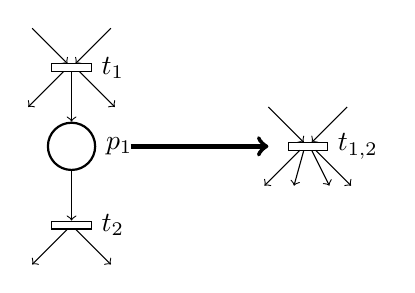
\begin{tikzpicture}
        \node[place, label=right:$p_1$](p)at(0,0){};
        \node[transition, rotate=90, label=below:$t_1$](t1)at(0,1){};
        \node[transition, rotate=90, label=below:$t_2$](t2)at(0,-1){};

        \draw[->](t1.180)--(p.90);
        \draw[->](p.270)--(t2.0);

        \draw[->](0.05,-1.05)--(0.5,-1.5);
        \draw[->](-0.05,-1.05)--(-0.5,-1.5);

        \draw[->](0.1,0.95)--(0.55,0.5);
        \draw[->](-0.1,0.95)--(-0.55,0.5);

        \draw[<-](0.05,1.05)--(0.5,1.5);
        \draw[<-](-0.05,1.05)--(-0.5,1.5);

        \draw[->, ultra thick](0.75,0)--(2.5,0);

        \node[transition, rotate=90, label=below:$t_{1,2}$](t3)at(3,0){};
        \draw[<-](3.05,0.05)--(3.5,0.5);
        \draw[<-](2.95,0.05)--(2.5,0.5);

        \draw[->](3.05,-0.05)--(3.275,-0.5);
        \draw[->](3.1,-0.05)--(3.55,-0.5);
        \draw[->](2.95,-0.05)--(2.825,-0.5);
        \draw[->](2.9,-0.05)--(2.45,-0.5);
    \end{tikzpicture}
\end{center}

Due posti si possono unire se sono collegati da un'unica transizione (abilitata), ed il peso degli archi entranti equivale il peso degli archi uscenti da essa. Il posto 
risultante contiene la somma dei gettoni presenti nei due posti:

\begin{center}
    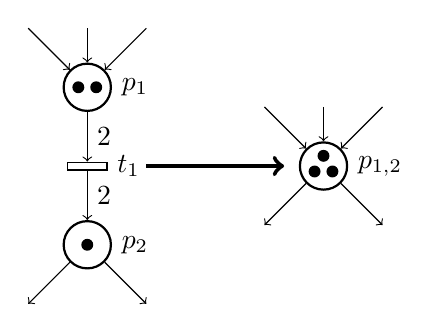
\begin{tikzpicture}
        \node[transition, rotate=90, label=below:$t_1$](t)at(0,0){};
        \node[place, tokens=2, label=right:$p_1$](p1)at(0,1){};
        \node[place, tokens=1, label=right:$p_2$](p2)at(0,-1){};

        \draw[->](p1.270)--(t.0)node[midway, right]{$2$};
        \draw[->](t.180)--(p2.90)node[midway, right]{$2$};

        \draw[->](0,1.75)--(p1.90);
        \draw[->](-0.75,1.75)--(p1.135);
        \draw[->](0.75,1.75)--(p1.45);

        \draw[->](p2.315)--(0.75,-1.75);
        \draw[->](p2.225)--(-0.75,-1.75);

        \draw[->, ultra thick](0.75,0)--(2.5,0);

        \node[place, tokens=3, label=right:$p_{1,2}$](p3)at(3,0){};

        \draw[->](3,0.75)--(p3.90);
        \draw[->](2.25,0.75)--(p3.135);
        \draw[->](3.75,0.75)--(p3.45);

        \draw[->](p3.315)--(3.75,-0.75);
        \draw[->](p3.225)--(2.25,-0.75);
    \end{tikzpicture}
\end{center}

Inoltre è possibile unire insieme transizioni o posti in parallelo, ovvero aventi gli stessi insieme di pre-set e post-set. 
In caso siano due posti connessi in parallelo, il posto risultante contiene la somma dei gettoni, mentre l'arco entrante al posto ha peso dato dalla somma dei pesi degli 
archi entranti nei due posti originali, analogamente per l'arco uscente dal posto risultante:
\begin{center}
    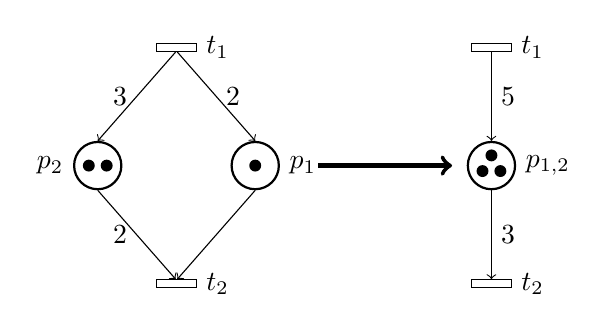
\begin{tikzpicture}
        \node[transition, rotate=90, label=below:$t_1$](t1)at(0,1.5){};
        \node[transition, rotate=90, label=below:$t_2$](t2)at(0,-1.5){};
        \node[place, tokens=1, label=right:$p_1$](p1)at(1,0){};
        \node[place, tokens=2, label=left:$p_2$](p2)at(-1,0){};

        \draw[->](t1.190)--(p1.90)node[midway, right]{$2$};
        \draw[->](t1.170)--(p2.90)node[midway, left]{$3$};
        \draw[<-](t2.350)--(p1.270)node[midway, right]{};
        \draw[<-](t2.10)--(p2.270)node[midway, left]{$2$};
        
        \draw[->,ultra thick](1.8,0)--(3.5,0);

        \node[transition, rotate=90, label=below:$t_1$](t3)at(4,1.5){};
        \node[transition, rotate=90, label=below:$t_2$](t4)at(4,-1.5){}; 
        \node[place, tokens=3, label=right:$p_{1,2}$](p3)at(4,0){};
        
        \draw[->](t3.180)--(p3.90)node[midway, right]{$5$};
        \draw[->](p3.270)--(t4.0)node[midway, right]{$3$};
    \end{tikzpicture}
\end{center}

In caso siano presenti due transizioni poste in parallelo, per unirle è necessario che gli archi entranti in entrambe le transizioni abbiano lo stesso peso, analogamente per 
le transizioni in uscita, in questo modo date due marcatura prima e dopo lo scatto di una delle due transizioni è impossibile distinguere quale delle due sia scattata, per cui 
si considerano come un'unica transizione:
\begin{center}
    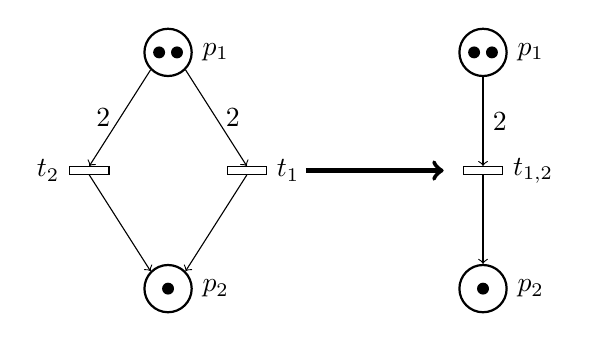
\begin{tikzpicture}
        \node[transition, rotate=90, label=below:$t_1$](t1)at(1,0){};
        \node[transition, rotate=90, label=above:$t_2$](t2)at(-1,0){};
        \node[place, tokens=2, label=right:$p_1$](p1)at(0,1.5){};
        \node[place, tokens=1, label=right:$p_2$](p2)at(0,-1.5){};

        \draw[->](p1.315)--(t1.0)node[midway, right]{$2$};
        \draw[->](p1.225)--(t2.0)node[midway, left]{$2$};
        \draw[->](t1.180)--(p2.45);
        \draw[->](t2.180)--(p2.135);

        \draw[->,ultra thick](1.75,0)--(3.5,0);

        \node[transition, rotate=90, label=below:$t_{1,2}$](t3)at(4,0){};
        \node[place, tokens=2, label=right:$p_1$](p3)at(4,1.5){};
        \node[place, tokens=1, label=right:$p_2$](p4)at(4,-1.5){};
        
        \draw[->](p3.270)--(t3.0)node[midway, right]{$2$};
        \draw[->](t3.180)--(p4.90);
    \end{tikzpicture}
\end{center}

Se in una rete è presente un autociclo, ovvero un posto o una transizione che presenta in pre-set e post-set lo stesso insieme, si può eliminare poiché non altera il 
comportamento della rete. 
In caso sia un posto in autociclo, se gli archi in entrata ed in uscita al posto hanno lo stesso peso, il numero di gettoni al suo interno rimane costante; se il peso dell'arco 
in entrata alla transizione è maggiore del numero dei gettoni interni al posto, la rete è morta, poiché quella transizione non sarà mai abilitata, quindi eliminandolo bisogna 
indicare che la rete sia morta, anche se la rete ridotta non lo è. Se il peso dell'arco in uscita è minore del peso dell'arco in entrata si raggiunge la stessa situazione, e 
la transizione diventa morta. 
\begin{center}
    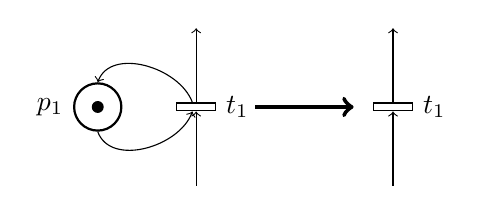
\begin{tikzpicture}
        \node[place, tokens=1, label=left:$p_1$](p1)at(0.25,0){};
        \node[transition, rotate=90, label=below:$t_1$](t1)at(1.5,0){};

        \draw[->](t1.40)to[out=110,in=70](p1.90);
        \draw[<-](t1.140)to[out=250,in=290](p1.270);

        \draw[->](1.5,-1)--(t1.180);
        \draw[->](t1.0)--(1.5,1);

        \draw[->,ultra thick](2.25,0)--(3.5,0);

        \node[transition, rotate=90, label=below:$t_1$](t2)at(4,0){};
        \draw[->](4,-1)--(t2.180);
        \draw[->](t2.0)--(4,1);
    \end{tikzpicture}
\end{center} 

Analogamente se è presenta una transizione avente in pre-set ed in post-set lo stesso posto, se il posto è $k-$limitato ed il peso del'arco entrante nella transizione è maggiore 
di $k$, allora quella transizione è morta. Se il peso degli archi entranti ed uscenti dalla transizione è uguale, non altera il numero dei gettoni nel posto associato. 
\begin{center}
    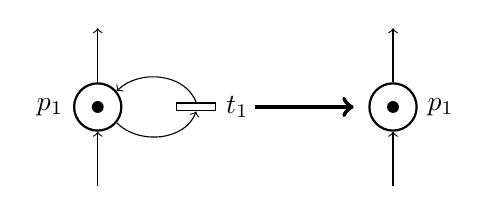
\begin{tikzpicture}
        \node[place, tokens=1, label=left:$p_1$](p1)at(0.25,0){};
        \node[transition, rotate=90, label=below:$t_1$](t1)at(1.5,0){};

        \draw[->](t1.0)to[out=110,in=45](p1.40);
        \draw[<-](t1.180)to[out=250,in=315](p1.320);

        \draw[->](0.25,-1)--(p1.270);
        \draw[->](p1.90)--(0.25,1);

        \draw[->,ultra thick](2.25,0)--(3.5,0);

        \node[place, tokens=1, label=right:$p_1$](t2)at(4,0){};
        \draw[->](4,-1)--(t2.270);
        \draw[->](t2.90)--(4,1);
    \end{tikzpicture}
\end{center} 

\subsection{Rappresentazione Algebrica}

\end{document}
